%%%----------------------------------------------------------
\chapter{Circle detection in binary dot images}
%%%----------------------------------------------------------

In this assignment we want to detect a circle which is embedded in a noisy binary image. To accomplish this task the RANSAC algorithm is used. 

\section{Algorithm}

At first the coordinates of all black pixels are collected and gathered in a list of points. Out of this list 3 points are randomly chosen and we make sure that no point is selected more than once.
With the help of these 3 points it is possible to determine the attributes of a circle which passes through them as shown in Figure \ref{CalculateCircle} following an article from Paul Borke\cite{PaulBorke2020}.

\begin{figure}
	\centering
	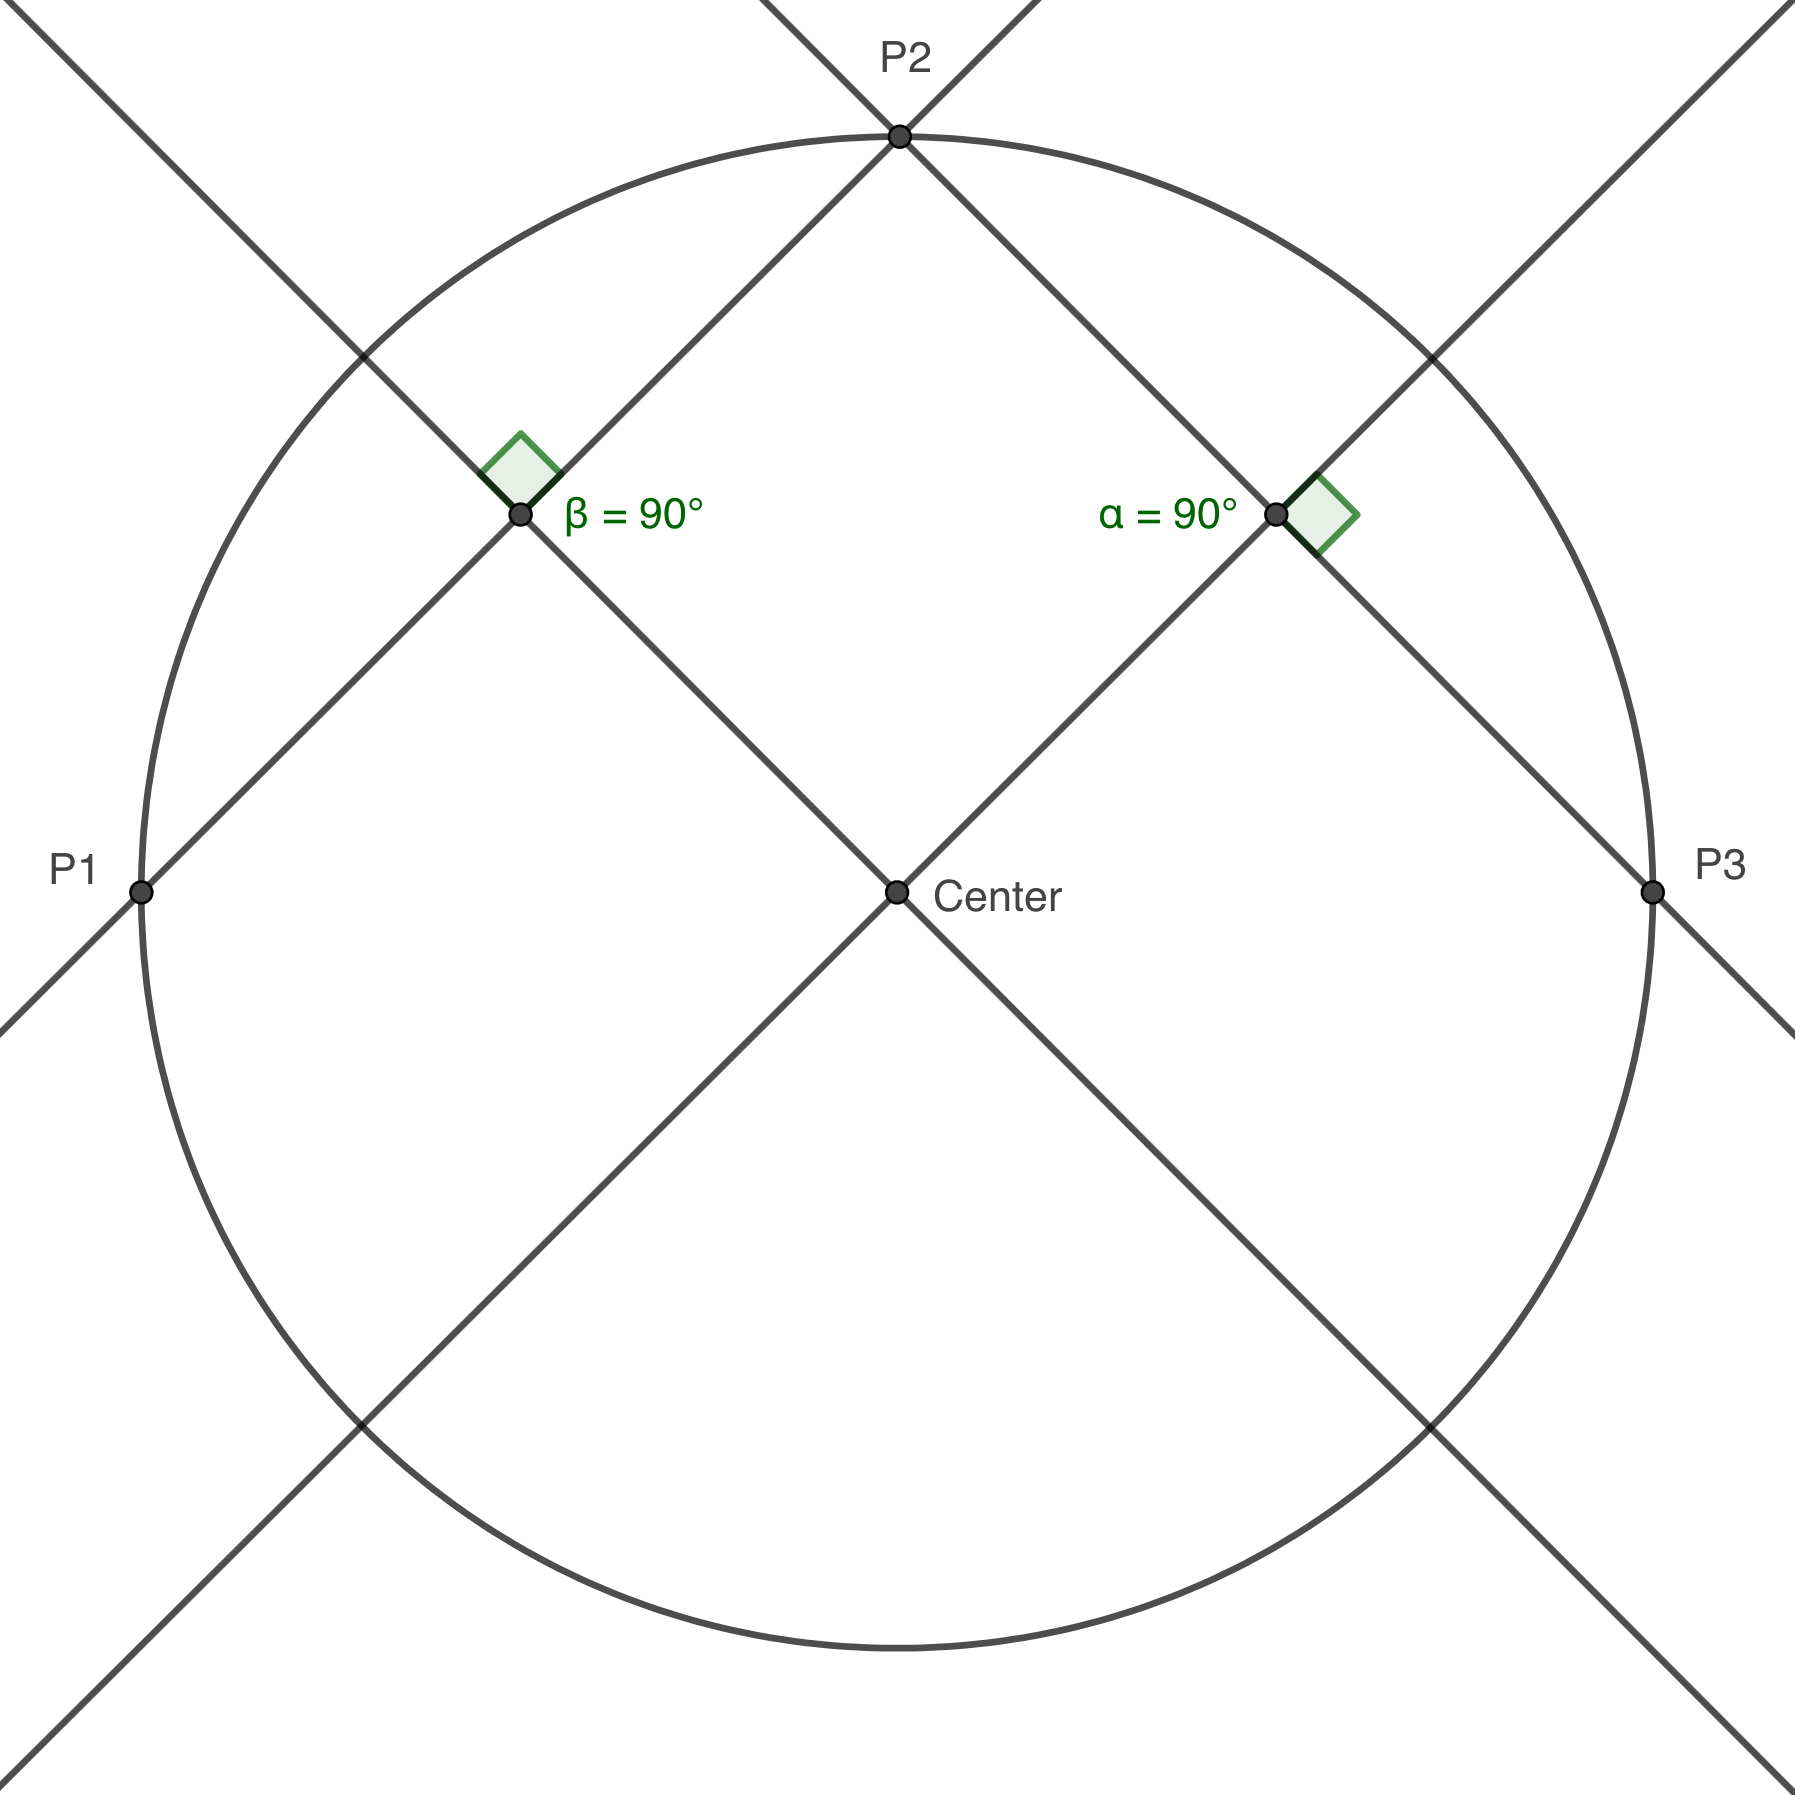
\includegraphics[width=.55\linewidth]{images/circlefrom3}
	\caption{Determine the center of a circle with 3 points.}
	\label{CalculateCircle}
\end{figure}

We form one line through the point $P_1$ and $P_2$ and another line through $P_2$ and $P_3$. The equation for these two lines are:
\begin{align*}
	y_a = m_a(x-x_1) + y_1\\
	y_b = m_b(x-x_2) + y_2
\end{align*}
$m$ is the slope for each line. So we have:
\begin{align}
	m_a& = \frac{y_2 - y_1}{x_2 - x_1}&
	m_b& = \frac{y_3 - y_2}{x_3 - x_2}
\end{align}
Now two lines perpendicular to the lines $y'_a$($P_1P_2$) and $y'_b$($P_2P_3$) going through the center between each point pair are created. The perpendicular of a line with slope $m$ has slope of $-1/m$. This results in following equations:
\begin{align}
	y'_a = -\frac{1}{m_a}(x-\frac{x_1 + x_2}{2}) + \frac{y_1 + y_2}{2}\label{perpendicular1}\\
	y'_b = -\frac{1}{m_b}(x-\frac{x_2 + x_3}{2}) + \frac{y_2 + y_3}{2}\label{perpendicular2}
\end{align}
The center of the circle is the intersection of these two perpendiculars. 
\begin{equation}
	x = \frac{m_am_b(y_1-y_3) + m_b(x_1+x_2) - m_a(x_2+x_3)}{2\cdot(m_b-m_a)}
\end{equation}
To calculate the y value of the center I substitute the x value into one of the two perpendiculars (\ref{perpendicular1}, \ref{perpendicular2}). The circle radius is determined by calculating the distance between the center point and one of the 3 originally chosen points.

There are 3 situations where a circle can not be calculated with just 3 points:
\begin{itemize}
	\item If all 3 points are collinear.
	\item If one point is selected more than once. This gets checked while selecting the points.
	\item If either line is vertical their slope would be infinite. To avoid that the order of the 3 points is rearranged if this is the case. 
\end{itemize}

After the circle is calculated the number of points on the circle gets determined. The distance between each detected point of the image and the center point of the circle is calculated and its difference to circle radius. If this difference is smaller than a certain threshold, the point is on the circle and it is saved in the point list of the circle. The threshold can be defined when the plugin is started.

The circle is saved as currently detected circle and this whole process gets repeated for a certain number of times which can be defined at the start of the plugin. After each iteration the number of points on the calculated circle is compared to the number of points on the currently detected circle. If the count is higher the detected circle gets replaced by the calculated circle.
 
As soon as this process was repeated for the defined number of times. The current detected circle gets drawn on the image in blue as well as all the points on it in red.

\begin{figure}
	\centering
	\begin{minipage}[t]{0.49\linewidth}
		\centering
			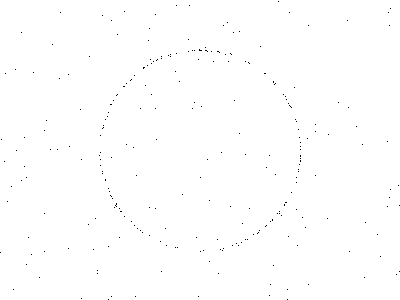
\includegraphics[width=.90\linewidth]{images/circle-test}
		\caption{Generated noisy binary image.}
	\end{minipage}
	\hfill
	\begin{minipage}[t]{0.49\linewidth}
		\centering
		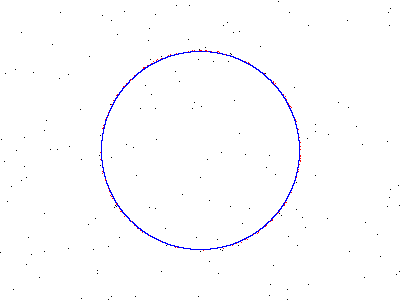
\includegraphics[width=.90\linewidth]{images/circle_result}
		\caption{The Detected circle after 25 iterations and a threshold distance of 1 from the circle}
	\end{minipage}
\end{figure}

\section{Research Question A}
\begin{itemize}
	\item The probability of selecting one point which lies on the circle is: $\frac{m}{n}$. If we choose 3 random points in a row we also need to make sure that we do not select the same point twice. This results in following formular:
	\begin{equation}
	P = \frac{m}{n} \cdot \frac{m-1}{n-1} \cdot \frac{m-2}{n-2}\label{probability}
	\end{equation}
	\item To calculate the number of random draws $n$ needed to select 3 circle points with a probability of 99\% we use following formular: $W = 1-(1-p)^n$ \cite{DanielaEder2020}. To calculate $p$  use the formular above (\ref{probability}) then solve the equation to get $n$.
	\begin{align}
	0.99& \geq 1 - (1-p)^n\\
	0.01& \geq (1-p)^n\\
	n& \geq \frac{\ln(0.01)}{\ln(1-p)}
	\end{align}
\end{itemize}

\section{Research Question B}

To detect multiple circles in one image a threshold for the number of points needs to be defined which are needed to be on a circle to be detected as a valid circle. If detected the circle is added to a list. To make sure that the same circle is not detected multiple times it has to be checked that there is no circle with the same center point and radius already in the list before adding it.